\subsection{Neural Architecture Codesign for Fast Physics Applications}
{{\footnotesize
\noindent Introduces a two-stage neural architecture codesign (NAC) pipeline combining global and local search,
quantization-aware training, and pruning to design efficient models for fast Bragg peak finding and
jet classification, synthesized for FPGA deployment with hls4ml. Achieves >30x reduction in BOPs
and sub-100 ns inference latency on FPGA.


\begin{description}[labelwidth=4cm, labelsep=1em, leftmargin=4cm, itemsep=0.1em, parsep=0em]
  \item[date:] 2025-01-09
  \item[version:] v1.0
  \item[last\_updated:] 2025-01
  \item[expired:] unknown
  \item[valid:] yes
  \item[valid\_date:] 2025-01-09
  \item[url:] \href{https://arxiv.org/abs/2501.05515}{https://arxiv.org/abs/2501.05515}
  \item[doi:] 10.48550/arXiv.2501.05515
  \item[domain:] Physics; Materials Science; Particle Physics
  \item[focus:] Automated neural architecture search and hardware-efficient model codesign for fast physics applications
  \item[keywords:]
    - neural architecture search
    - FPGA deployment
    - quantization
    - pruning
    - hls4ml
  \item[licensing:] Via Fermilab
  \item[task\_types:]
    - Classification
    - Peak finding
  \item[ai\_capability\_measured:]
    - Hardware-aware model optimization; low-latency inference
  \item[metrics:]
    - Accuracy
    - Latency
    - Resource utilization
  \item[models:]
    - NAC-based BraggNN
    - NAC-optimized Deep Sets (jet)
  \item[ml\_motif:]
    - Real-time, Image/CV
  \item[type:] Framework
  \item[ml\_task:]
    - Supervised Learning
  \item[solutions:] Solution details are described in the referenced paper or repository.
  \item[notes:] Demonstrated two case studies (materials science, HEP); pipeline and code open-sourced.

  \item[contact.name:] Jason Weitz (UCSD), Nhan Tran (FNAL)
  \item[contact.email:] unknown
  \item[results.links.name:] ChatGPT LLM
  \item[fair.reproducible:] Yes (nac-opt, hls4ml)
  \item[fair.benchmark\_ready:] False
  \item[id:] neural\_architecture\_codesign\_for\_fast\_physics\_applications
  \item[Citations:] \cite{weitz2025neuralarchitecturecodesignfast}
\end{description}

{\bf Ratings:} ~ \\

\begin{tabular}{p{0.15\textwidth} p{0.07\textwidth} p{0.7\textwidth}}
\hline
Rating & Value & Reason \\
\hline
dataset & 2 & Simulated datasets referenced but not publicly available or FAIR-compliant
 \\
documentation & 4 & Detailed paper and tools described; open repo planned but not yet complete
 \\
metrics & 5 & Clear, quantitative metrics aligned with task goals and hardware evaluation
 \\
reference\_solution & 4 & Models tested on hardware with source code references; full training pipeline not yet released
 \\
software & 3 & Toolchain (hls4ml, nac-opt) described but not yet containerized or fully packaged
 \\
specification & 5 & Fully specified task with constraints and target deployment; includes hardware context
 \\
\hline
\end{tabular}

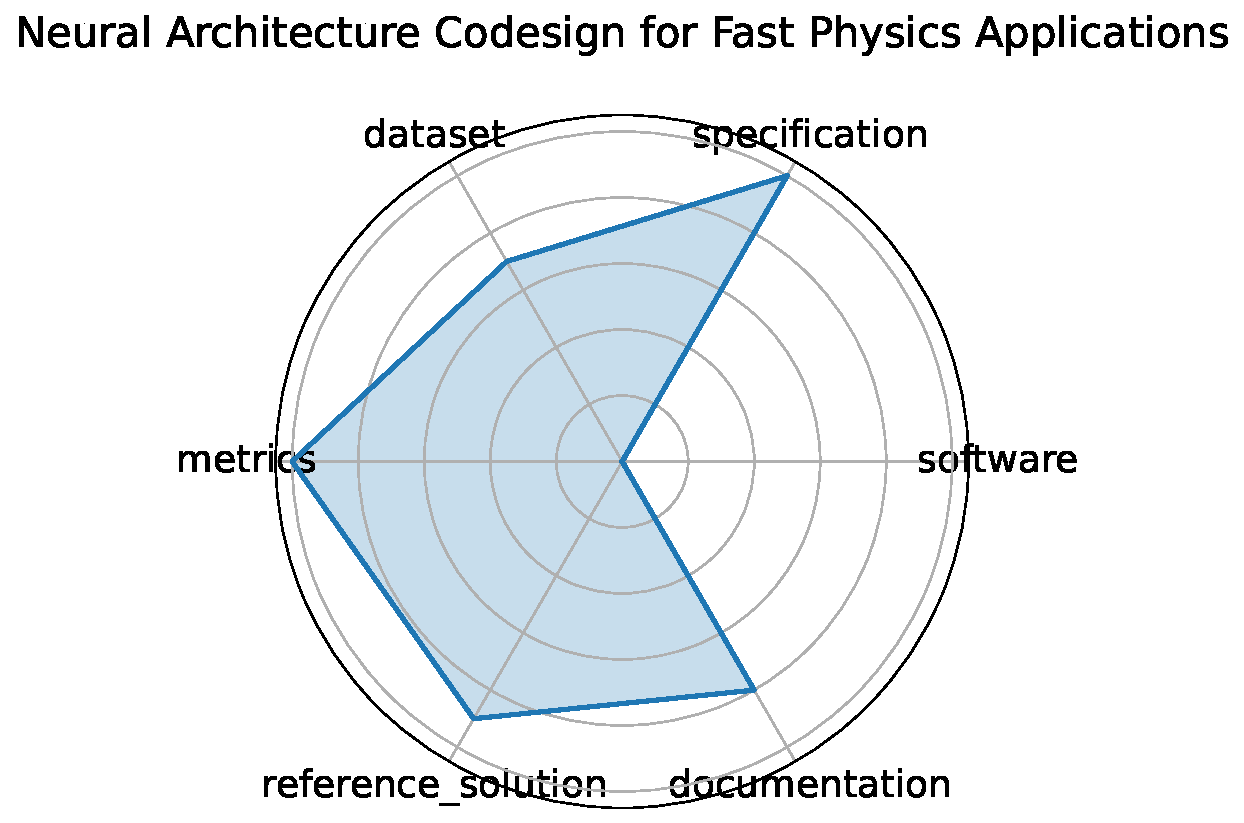
\includegraphics[width=0.2\textwidth]{neural_architecture_codesign_for_fast_physics_applications_radar.pdf}
}}
\clearpage